%
% This is a borrowed LaTeX template file for lecture notes for CS267,
% Applications of Parallel Computing, UCBerkeley EECS Department.
% Now being used for CMU's 10725 Fall 2012 Optimization course
% taught by Geoff Gordon and Ryan Tibshirani.  When preparing 
% LaTeX notes for this class, please use this template.
%
% To familiarize yourself with this template, the body contains
% some examples of its use.  Look them over.  Then you can
% run LaTeX on this file.  After you have LaTeXed this file then
% you can look over the result either by printing it out with
% dvips or using xdvi. "pdflatex template.tex" should also work.
%

\documentclass[twoside]{article}
\setlength{\oddsidemargin}{0.25 in}
\setlength{\evensidemargin}{-0.25 in}
\setlength{\topmargin}{-0.6 in}
\setlength{\textwidth}{6.5 in}
\setlength{\textheight}{8.5 in}
\setlength{\headsep}{0.75 in}
\setlength{\parindent}{0 in}
\setlength{\parskip}{0.1 in}

%
% ADD PACKAGES here:
%

\usepackage{amsmath,amsfonts,graphicx}

%
% The following commands set up the lecnum (lecture number)
% counter and make various numbering schemes work relative
% to the lecture number.
%
\newcounter{lecnum}
\renewcommand{\thepage}{\thelecnum-\arabic{page}}
\renewcommand{\thesection}{\thelecnum.\arabic{section}}
\renewcommand{\theequation}{\thelecnum.\arabic{equation}}
\renewcommand{\thefigure}{\thelecnum.\arabic{figure}}
\renewcommand{\thetable}{\thelecnum.\arabic{table}}

%
% The following macro is used to generate the header.
%
\newcommand{\lecture}[4]{
   \pagestyle{myheadings}
   \thispagestyle{plain}
   \newpage
   \setcounter{lecnum}{#1}
   \setcounter{page}{1}
   \noindent
   \begin{center}
   \framebox{
      \vbox{\vspace{2mm}
    \hbox to 6.28in { {\bf EE402 - Discrete Time Systems
	\hfill Spring 2018} }
       \vspace{4mm}
       \hbox to 6.28in { {\Large \hfill Lecture #1 \hfill} }
       \vspace{2mm}
       \hbox to 6.28in { {\it Lecturer: #2 \hfill } }
      \vspace{2mm}}
   }
   \end{center}
   \markboth{Lecture #1}{Lecture #1}

   \vspace*{4mm}
}
%
% Convention for citations is authors' initials followed by the year.
% For example, to cite a paper by Leighton and Maggs you would type
% \cite{LM89}, and to cite a paper by Strassen you would type \cite{S69}.
% (To avoid bibliography problems, for now we redefine the \cite command.)
% Also commands that create a suitable format for the reference list.
\renewcommand{\cite}[1]{[#1]}
\def\beginrefs{\begin{list}%
        {[\arabic{equation}]}{\usecounter{equation}
         \setlength{\leftmargin}{2.0truecm}\setlength{\labelsep}{0.4truecm}%
         \setlength{\labelwidth}{1.6truecm}}}
\def\endrefs{\end{list}}
\def\bibentry#1{\item[\hbox{[#1]}]}

%Use this command for a figure; it puts a figure in wherever you want it.
%usage: \fig{NUMBER}{SPACE-IN-INCHES}{CAPTION}
\newcommand{\fig}[3]{
			\vspace{#2}
			\begin{center}
			Figure \thelecnum.#1:~#3
			\end{center}
	}
% Use these for theorems, lemmas, proofs, etc.
\newtheorem{theorem}{Theorem}[lecnum]
\newtheorem{lemma}[theorem]{Lemma}
\newtheorem{proposition}[theorem]{Proposition}
\newtheorem{claim}[theorem]{Claim}
\newtheorem{corollary}[theorem]{Corollary}
\newtheorem{definition}[theorem]{Definition}
\newenvironment{proof}{{\bf Proof:}}{\hfill\rule{2mm}{2mm}}

% **** IF YOU WANT TO DEFINE ADDITIONAL MACROS FOR YOURSELF, PUT THEM HERE:

\begin{document}

% Lecture Details
\lecture{5}{Asst. Prof. M. Mert Ankarali}


Let's remember the idealized and simplified block-diagram structure 
a discrete-time control system (See Fig.~\ref{fig:introblock})

\begin{figure}[h]
    \centering
      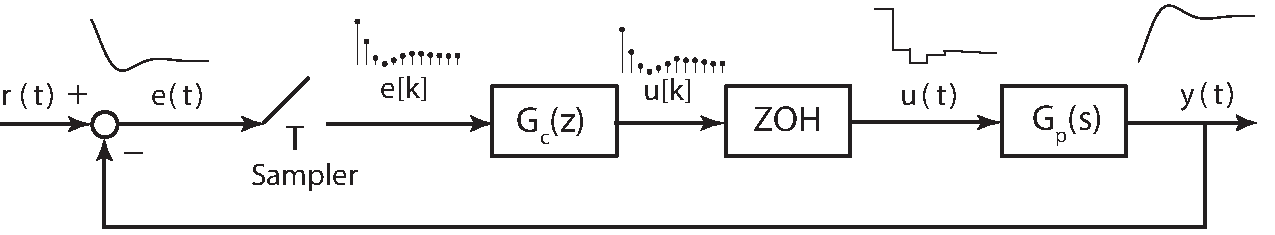
\includegraphics[width=0.99\textwidth]{idealblock}
    \caption{Block diagram of an LTI discrete-time control system}
    \label{fig:introblock}
\end{figure}

Loop contains both continuous-time and discrete-time signals and
blocks.

\begin{itemize}
  \item We can treat the system as a completely discrete-time
  system. We technically restrict ourselves into sampled time instants
  (in this course we will fundementally follow this path)
\item Alternatively, we can use continuous time signals (as much as
  possible) and deal with starred versions of signals and starred
  Laplace transform (In original--with star notation--notes, I sometimes follow this path).
\end{itemize}

\section{Data Hold Operation}

Data-Hold operation is an idealized model of
a DAC device which converts a digital signal 
to an analog signal. In terms of the terminology used 
in this class, Data-Hold operation is the process of 
obtaining a CT signal $h(t)$ from a DT sequence.
A general data-hold operation block circuit is shown 
below
%
    \begin{center}
\begin{minipage}[h]{0.5\linewidth}
    \begin{center}
      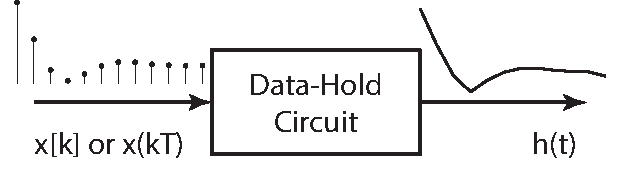
\includegraphics[width=\textwidth]{holdgeneral}
    \end{center}
\end{minipage}
    \end{center}
%
Simplest and most dominantly used (I have never seen a practical
usage of other hold operations) hold circuit/operation is 
the zero-order-hold (ZOH). Basically, at each time instant $k T$
ZOH ``samples'' the input $x[k]$ or $x(kT)$ and ``holds'' this value 
at the output until the next sampling event. Mathematically, 
%
\begin{align*}
  h(kT + t) = x(kT) = x[k], \ \mathrm{for} \ 0 \leq t < T 
\end{align*}
%
The figure below illustrates a serios connection of an ideal
CT-DT sampler and an ideal ZOH block. 
%
    \begin{center}
\begin{minipage}[h]{0.7\linewidth}
    \begin{center}
      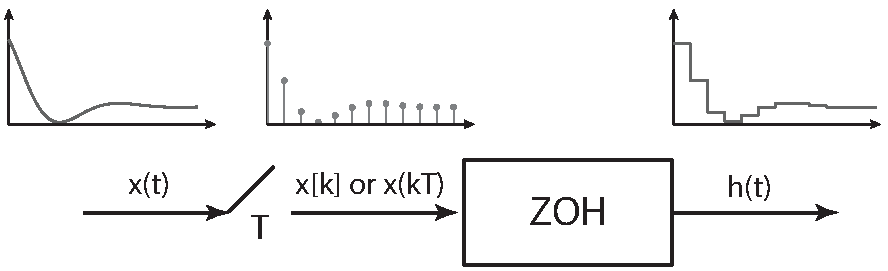
\includegraphics[width=\textwidth]{zoh1}
    \end{center}
\end{minipage}
    \end{center}
%
Let's assume that $x(t)$ is a strictly causal signal, then from the
definition of ZOH we can express $h(t)$ in terms of $x(t)$ (or
$x[k]$, $x(kT)$) as
%
\begin{align*}
h(t) &= x(0) \left[ u(t) - u(t-T) \right] + x(T) \left[ u(t-T) - u(t-2T)
  \right] + x(2T) \left[ u(t-2T) - u(t-3T) \right] + \cdots
\\
h(t) &= \sum\limits_{k=0}^{\infty} x(kT) \left[ u(t-kT) - u(t-(k+1)T) \right] 
\end{align*}
%
where $u(t)$ is the unit-step function.

If we take the Laplace transform of $h(t)$, we obtain
%
\begin{align*}
\mathcal{L} \lbrace h(t) \rbrace &= \sum\limits_{k=0}^{\infty} x(kT)
                                   \mathcal{L} \left\lbrace  \left[
                                   u(t-kT) - u(t-(k+1)T) \right]
                                   \right\rbrace
\\
&= \sum\limits_{k=0}^{\infty} x(kT) \left[
                                   \frac{e^{-k T s}}{s} -
  \frac{e^{-(k+1) T s}}{s}\right]
\\
H(s) &= \frac{1 - e^{-Ts}}{s} \sum\limits_{k=0}^{\infty} x(kT) e^{-k T s} =
  \frac{1 - e^{-Ts}}{s} \sum\limits_{k=0}^{\infty} x[k] e^{-k T s}
\end{align*}

\subsection*{Z-transform \& ZOH}

When analyzing the discrete time control systems,
we will (frequently) need to compute the Z-transform of sampled
signals, for which the Laplace transform involves the 
term $\left( 1 - e^{-T s}  
\right)$. 

Let $\mathcal{L} \lbrace x(t) \rbrace=  X(s) = \left( 1 - e^{-T s} \right) G(s)$. Now let's analyze the z-transform of the sampled version 
of the signal, i.e. $X(z) = \mathcal{Z} \lbrace x(k T) \rbrace$.
First let's find $x(t)$ from $X(z)$
%
\begin{align*}
x(t) &= \mathcal{L}^{-1} \lbrace X(s) \rbrace = \mathcal{L}^{-1} \left\lbrace \left( 1 - e^{-T s} \right) G(s) \right\rbrace 
=  \mathcal{L}^{-1} \left\lbrace G(s) \right\rbrace
- \mathcal{L}^{-1} \left\lbrace e^{-Ts} G(s) \right\rbrace
 \end{align*}
%
Let $g(t) = \mathcal{L}^{-1} \left\lbrace G(s)
\right\rbrace$ then
%
\begin{align*}
x(t) &= g(t) - g(t-T)
 \end{align*}
%
$x(kT)$ and $x[k]$ takes the form
%
\begin{align*}
x(k T) &= g(k T) - g(kT -T)
\\
x[k] &= \hat{g}[k] - \hat{g}[k-1]
 \end{align*}
%
Then $X(z)$ takes the form
%
\begin{align*}
X(z) &= \left( 1 - z^{-1} \right) G(z) 
 \end{align*}
%
where $G(z) = \mathcal{Z} \left\lbrace \left[ \mathcal{L}^{-1}
  \left\lbrace G(s) \right\rbrace \right]^* \right\rbrace$ and $*$ is the sampling operation.
In the textbook this notation is shortened to have
$G(z) = \mathcal{Z} \left\lbrace G(s) \right\rbrace$.
After that we have
%
\begin{align*}
X(z) &= \left( 1 - z^{-1} \right) \mathcal{Z} \left\lbrace G(s) \right\rbrace
 \end{align*}
%

\textbf{Example 1.} Obtain the z transform of $x(kT)$ where $T=1$ and $X(s)$ is
given as
%
\begin{align*}
  X(s) = \frac{1 - e^{-s}}{s} \frac{1}{s+1}
\end{align*}
%
\textbf{Solution:}
%
\begin{align*}
  X(z) &= \left( 1 - z^{-1} \right) \mathcal{Z} \left\lbrace \frac{1}{s(s+1)}
  \right\rbrace
= \left( 1 - z^{-1} \right) \mathcal{Z} \left\lbrace \frac{1}{s} -
  \frac{1}{s+1} \right\rbrace
\\
&= \frac{z-1}{z} \left( \frac{z}{z-1} - \frac{z}{z-e^{-1}}  \right)
= 1 - \frac{z-1}{z-e^{-1}} \\
X(z) &= \frac{1-e^{-1}}{z-e^{-1}}
\end{align*}

\section{Discretization of CT TF under ZOH and Ideal Sampling Operators}

The figure below illustrates an open loop fundamental digital control control system 
that is composed of a CT plant, $G(s)$, a ZOH operator, and an ideal syncronous sampler. 
Our goal is to find a DT (z-domain) transfer function between the discrete-time input signal, 
$x[k]$ and the discrete-time output signal, $y[k]$, i.e. $ frac{Y(z)}{X(z)}$ .

%
    \begin{center}
\begin{minipage}[h]{0.99\linewidth}
    \begin{center}
      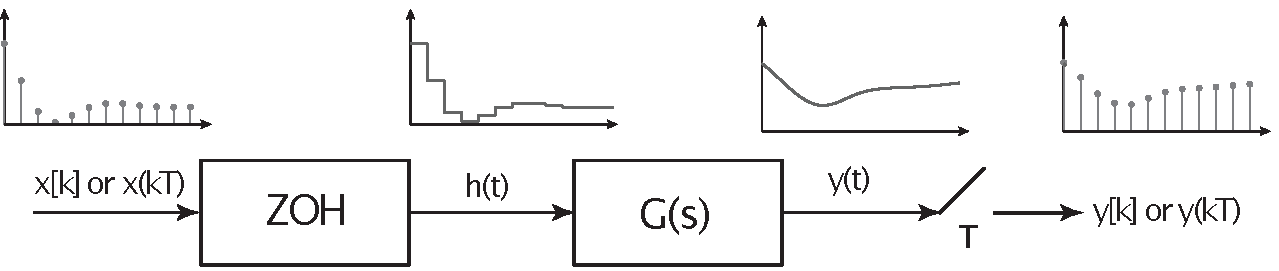
\includegraphics[width=\textwidth]{DCS}
    \end{center}
\end{minipage}
    \end{center}
%
Let's first concentrate on input--output dynamics of $G(s)$
%
\begin{align*}
Y(s) &= G(s)  H(s)
\\
&= G(s)  \frac{1 - e^{-Ts}}{s} \sum\limits_{k=0}^{\infty} x[k] e^{-k T s}
\\
&= \left( 1 - e^{-Ts} \right)  \frac{G(s) }{s} \sum\limits_{k=0}^{\infty} x[k] e^{-k T s}
\\
&= \left( 1 - e^{-Ts} \right)  
\hat{G}(s) \sum\limits_{k=0}^{\infty} x[k] e^{-k T s}
\end{align*}
%
where $\hat{G}(s)$ is also the Laplace transform of the step-response of $G(s)$. 
Let $P(s) =  \hat{G}(s) \sum\limits_{k=0}^{\infty} x[k] e^{-k T s}$, and try to derive
$P(z) = \mathcal{Z} \left\lbrace P(s) \right\rbrace$. First take the inverse Laplace
transform of the expression
%
\begin{align*}
p(t) &= \mathcal{L}^{-1} \left\lbrace \hat{G}(s) \sum\limits_{k=0}^{\infty} x[k] e^{-k T s} \right\rbrace
= \sum\limits_{k=0}^{\infty} x[k] \mathcal{L}^{-1} \left\lbrace \hat{G}(s) e^{-k T s} \right\rbrace
\\
&= \sum\limits_{k=0}^{\infty} x[k] \hat{g}(t - k T) 
\end{align*}
%
If we limit ourselves to causal $g(t)$ case and sample $p(t)$, we will obtain
%
\begin{align*}
p( n T) = p[k] =  \sum\limits_{k=0}^{n} x[k] \hat{g}( \left(n - k\right) T) = \sum\limits_{k=0}^{n} x[k] \hat{g}[ n - k ]
\end{align*}
%
Note that this is the expression of the discrete-time convolution, and thus we can infer the followings 
%
\begin{align*}
p(n T) &= \hat{g}(nT) \ast x(nT) = x(nT) \ast \hat{g}(nT) 
\\
p[n] &= \hat{g}[n] \ast x[n] = x[n] \ast \hat{g}[n] 
\\
P(z) &= \hat{G}(z) X(z)
\end{align*}
%
If we use the derivation that we found previously regarding the 
Z-transform of sampled signals, for which the Laplace transform involves the 
term $\left( 1 - e^{-T s} \right)$, we can compute $Y(z)$ as 
% 
\begin{align*}
Y(z) &= \left( 1 - z^{-1} \right) P(z) = \left( 1 - z^{-1} \right) 
\hat{G}(z) X(z)
\\
G_d(z) = \frac{Y(z)}{X(z)} &= \left( 1 - z^{-1} \right) \hat{G}(z) \quad \mathrm{where} \ \hat{G}(z) = \mathcal{Z} \left\lbrace 
\frac{G(s)}{s} \right\rbrace
\end{align*}
%
We call $G_d(z)$ as the discretized transfer function of $G(s)$
under ZOH and ideal sampling operators. The result is pretty interesting: the impulse response of the
``discretized'' system is obtained by sampling the step response function of original the 
continuous time system. 


% **** This ENDS THE EXAMPLES. DON'T DELETE THE FOLLOWING LINE:
\end{document}